
\newcommand{\GrundlegendeLaufzeitenAbhaengigVonDerArraygroesseMesszielFolien}{

    \begin{frame}[shrink=10]{Grundlegende Laufzeiten abhängig von der Arraygröße (sequenziell)}
        \centering
        \resizebox{0.99\textwidth}{!}{%
            \centering
            \begin{minipage}{\linewidth}
                \begin{minipage}{0.5\linewidth}
                    \centering
                    \GrundlegendeLaufzeitenAbhaengigVonDerArraygroesseDiagrammA
                    \captionof{figure}[Grundlegende Laufzeit der Sortierverfahren (Arraygröße 1 - 400M)]{}
                    \label{fig:GrundlegendeLaufzeitenAbhaengigVonDerArraygroesseDiagrammA}
                \end{minipage}%
                \begin{minipage}{0.5\linewidth}
                    \centering
                    \GrundlegendeLaufzeitenAbhaengigVonDerArraygroesseDiagrammB
                    \captionof{figure}[Grundlegende Laufzeit der Sortierverfahren (Arraygröße 25M - 400M, logarithmische Achsen)]{}
                    \label{fig:GrundlegendeLaufzeitenAbhaengigVonDerArraygroesseDiagrammB}
                \end{minipage}
            \end{minipage}
        }
    \end{frame}

    \begin{frame}[shrink=10]{Grundlegende Laufzeiten abhängig von der Arraygröße (sequenziell)}
        \begin{minipage}{\linewidth}
            \centering
            \GrundlegendeLaufzeitenAbhaengigVonDerArraygroesseDiagrammC
            \captionof{figure}[Grundlegende Laufzeit der Sortierverfahren (Arraygröße 1 - 800k, logarithmische Achsen)]{}
            \label{fig:GrundlegendeLaufzeitenAbhaengigVonDerArraygroesseDiagrammC}
        \end{minipage}
    \end{frame}

}

\newcommand{\EinflussDesListentypsMesszielFolien}{

    \begin{frame}{Einfluss des Listentyps (sequenziell)}
        \resizebox{0.99\textwidth}{!}{
            \begin{minipage}{\linewidth}
                \centering
                \EinflussDesListentypsDiagrammA
                \captionof{figure}[Laufzeit der Sortierverfahren (Arraygröße 1 - 400M)]{}
                \label{fig:EinflussDesListentypsDiagrammA}
            \end{minipage}

            \begin{minipage}{\linewidth}
                \centering
                \EinflussDesListentypsDiagrammB
                \captionof{figure}[Laufzeit der Sortierverfahren (Arraygröße 25M - 400M, logarithmische Achsen)]{}
                \label{fig:EinflussDesListentypsDiagrammB}
            \end{minipage}
        }
    \end{frame}

    \begin{frame}{Einfluss des Listentyps (sequenziell)}
        \resizebox{0.99\textwidth}{!}{
            \begin{minipage}{\linewidth}
                \centering
                \EinflussDesListentypsDiagrammB
                \captionof{figure}[Laufzeit der Sortierverfahren (Arraygröße 25M - 400M, logarithmische Achsen)]{}
                \label{fig:EinflussDesListentypsDiagrammB}
            \end{minipage}
        }
    \end{frame}

    \begin{frame}[shrink=10]{Einfluss des Listentyps (sequenziell)}
        \resizebox{0.99\textwidth}{0.5\textheight}{
            \begin{minipage}{\linewidth}
                \centering
                \EinflussDesListentypsDiagrammC
                \captionof{figure}[Laufzeit der Sortierverfahren (Arraygröße 1 - 400M, logarithmische Achsen)]{}
                \label{fig:EinflussDesListentypsDiagrammC}
            \end{minipage}
        }
    \end{frame}

    % \begin{frame}[shrink=10]{Einfluss des Listentyps (sequenziell)}
    %     \resizebox{0.99\textwidth}{0.65\textheight}{
    %         \begin{minipage}{\linewidth}
    %             \centering
    %             \EinflussDesListentypsDiagrammC
    %             \captionof{figure}[Laufzeit der Sortierverfahren (Arraygröße 1 - 400M, logarithmische Achsen)]{}
    %             \label{fig:EinflussDesListentypsDiagrammC}
    %         \end{minipage}
    %     }
    % \end{frame}

}

\newcommand{\TiefenbasierteThreadErzeugungMesszielFolien}{
    \begin{frame}[shrink=15]{Tiefenbasierte Thread-Erzeugung}
        \begin{minipage}{\linewidth}
            \centering
            \TiefenbasierteThreadErzeugungDiagrammB
            \captionof{figure}[Strong Scaling (Tiefenbasierte Thread-Erzeugung)]{Strong Scaling (Tiefenbasierte Thread-Erzeugung): Die gestrichelten Linien zeigen die theoretisch zu erwartenden Laufzeitverbesserungen. Quicksort kann diese Verbesserung nur im Best-Case erreichen.
                T = Tiefenbasierte Thread-Erzeugung
            }
            \label{fig:TiefenbasierteThreadErzeugungDiagrammB}
        \end{minipage}
    \end{frame}

    \begin{frame}[shrink=15]{Tiefenbasierte Thread-Erzeugung}
        \begin{minipage}{\linewidth}
            \centering
            \TiefenbasierteThreadErzeugungDiagrammC
            \captionof{figure}[Weak Scaling (Tiefenbasierte Thread-Erzeugung)]{Weak Scaling (Tiefenbasierte Thread-Erzeugung): Die gestrichelten Linien zeigen die theoretisch zu erwartenden Laufzeitverbesserungen. Quicksort kann diese Verbesserung nur im Best-Case erreichen.
                T = Tiefenbasierte Thread-Erzeugung
            }
            \label{fig:TiefenbasierteThreadErzeugungDiagrammC}
        \end{minipage}
    \end{frame}

    \begin{frame}[shrink=10]{Tiefenbasierte Thread-Erzeugung}
        \resizebox{0.99\textwidth}{0.5\textheight}{
            \begin{minipage}{\linewidth}
                \centering
                \TiefenbasierteThreadErzeugungDiagrammA
                \captionof{figure}[Laufzeit der Sortierverfahren (Tiefenbasierte Thread-Erzeugung, Arraygröße 1 - 400M)]{
                    T16 = Tiefenbasierte Thread-Erzeugung mit 16 Threads
                }
                \label{fig:TiefenbasierteThreadErzeugungDiagrammA}
            \end{minipage}
        }
    \end{frame}
}

\newcommand{\WorkerthreadsMesszielFolien}{
    \begin{frame}{Workerthreads}
        \begin{minipage}{\linewidth}
            \centering
            \initZeitenDiagrammA
            \captionof{figure}[Laufzeit der Sortierverfahren bei einer Arraygröße von 16 Elementen]{Dieses Diagramm dient der Abschätzung der durch Threads entstehenden Overheads.
                T = Tiefenbasierte Thread-Erzeugung,
                WT = Worker-Thread-Variante
            }
            \label{fig:initZeitenDiagrammA}
        \end{minipage}
    \end{frame}

    \begin{frame}[shrink=20]{Workerthreads}
        \begin{minipage}{\linewidth}
            \centering
            \WorkerthreadsDiagrammB
            \captionof{figure}[Strong Scaling (Worker-Thread)]{Strong Scaling (Worker-Thread): Die gestrichelten Linien zeigen die theoretisch zu erwartenden Laufzeitverbesserungen.
                WT = Worker-Thread-Variante
            }
            \label{fig:WorkerthreadsDiagrammB}
        \end{minipage}
    \end{frame}

    \begin{frame}[shrink=20]{Workerthreads}
        \begin{minipage}{\linewidth}
            \centering
            \WorkerthreadsDiagrammC
            \captionof{figure}[Weak Scaling (Worker-Thread)]{Weak Scaling (Worker-Thread): Die gestrichelten Linien zeigen die theoretisch zu erwartenden Laufzeitverbesserungen.
                WT = Worker-Thread-Variante
            }
            \label{fig:WorkerthreadsDiagrammC}
        \end{minipage}
    \end{frame}

    \begin{frame}[shrink=10]{Workerthreads}
        \resizebox{0.99\textwidth}{0.5\textheight}{
            \begin{minipage}{\linewidth}
                \centering
                \WorkerthreadsDiagrammA
                \captionof{figure}[Laufzeit der Sortierverfahren (Worker-Thread, Arraygröße 1 - 400M)]{
                    WT16 = Worker-Thread-Variante mit 16 Worker-Threads
                }
                \label{fig:WorkerthreadsDiagrammA}
            \end{minipage}
        }
    \end{frame}
}

\newcommand{\EinflussDesDatentypsMesszielFolien}{
    \begin{frame}[shrink=15]{Einfluss des Datentyps der Liste (String)}
        \begin{minipage}{\linewidth}
            \centering
            \EinflussDesDatentypsDiagrammB
            \captionof{figure}[Strong Scaling (String)]{Strong Scaling (String): Die gestrichelten Linien zeigen die theoretisch zu erwartenden Laufzeitverbesserungen.
                T = Tiefenbasierte Thread-Erzeugung,
                WT = Worker-Thread-Variante
            }
            \label{fig:EinflussDesDatentypsDiagrammB}
        \end{minipage}
    \end{frame}

    \begin{frame}[shrink=15]{Einfluss des Datentyps der Liste (String)}
        \begin{minipage}{\linewidth}
            \centering
            \EinflussDesDatentypsDiagrammC
            \captionof{figure}[Weak Scaling (String)]{Weak Scaling (String): Die gestrichelten Linien zeigen die theoretisch zu erwartenden Laufzeitverbesserungen.
                T = Tiefenbasierte Thread-Erzeugung,
                WT = Worker-Thread-Variante
            }
            \label{fig:EinflussDesDatentypsDiagrammC}
        \end{minipage}
    \end{frame}

    \begin{frame}[shrink=10]{Einfluss des Datentyps der Liste (String)}
        \resizebox{0.99\textwidth}{0.5\textheight}{
            \begin{minipage}{\linewidth}
                \centering
                \EinflussDesDatentypsDiagrammA
                \captionof{figure}[Laufzeit der Sortierverfahren (String, Arraygröße 1 - 80M)]{
                    T16 = Tiefenbasierte Thread-Erzeugung mit 16 Threads,
                    WT16 = Worker-Thread-Variante mit 16 Worker-Threads
                }
                \label{fig:EinflussDesDatentypsDiagrammA}
            \end{minipage}
        }
    \end{frame}
}

\newcommand{\InkrementArrayfolien}{
    \resizebox{0.66\textwidth}{4.5cm}{%
        \begin{minipage}{\textwidth}
            \centering
            % Zeile 1
            \begin{minipage}{0.5\textwidth}
                \centering \InkrementArrayDiagrammA
                \captionof{figure}[Inkrement-Array ($2\times$ Geschwindigkeit)]{
                    Zeigt, ab welcher Arraygröße zum ersten Mal die halbe Laufzeit gegenüber der sequentiellen Laufzeit erreicht wird.
                }
                \label{fig:InkrementArrayDiagrammGeschwindigkeitssteigerung}
            \end{minipage}%
            \begin{minipage}{0.5\textwidth}
                \centering \InkrementArrayDiagrammB
                \captionof{figure}[Inkrement-Array (Strong Scaling: Laufzeit bei Arraygröße $2^{21}$)]{}
                \label{fig:InkrementArrayDiagrammStrongScalingA}
            \end{minipage}%
            \begin{minipage}{0.5\textwidth}
                \centering \InkrementArrayDiagrammE
                \captionof{figure}[Inkrement-Array (Weak Scaling {\small (Start-Größe $2^{21}$)})]{}
            \end{minipage}

            \par\vspace{1em}

            \begin{minipage}{0.5\textwidth}
                \centering \InkrementArrayDiagrammD
                \captionof{figure}[Inkrement-Array (Laufzeit bei Arraygröße 16)]{
                    Zeigt die Overheads, die durch Threads entstehen.
                }
            \end{minipage}%
            \begin{minipage}{0.5\textwidth}
                \centering \InkrementArrayDiagrammC
                \captionof{figure}[Inkrement-Array (Strong Scaling: Laufzeit bei Arraygröße $2^{31}$)]{}
                \label{fig:InkrementArrayDiagrammStrongScalingB}
            \end{minipage}%
            \begin{minipage}{0.5\textwidth}
                \centering \InkrementArrayDiagrammF
                \captionof{figure}[Inkrement-Array (Arraygröße verdoppeln (16 Threads))]{}
            \end{minipage}
        \end{minipage}
    }
}

\newcommand{\Baumfolien}{

    \begin{frame}{Implementierungsvarianten}
        Bildlich gesprochen lässt sich Mergesort als balancierter und Quicksort als unbalancierter binärer Baum darstellen.
        Während die tiefenbasierte Thread-Erzeugung bis zu einer festen Ebene bei Mergesort zu einer optimalen Auslastung führt, resultiert dies bei Quicksort in einer schlechten Lastverteilung.
        Im Gegensatz dazu ermöglicht die Work-Stealing-Variante, dass freie Threads Aufgaben aus anderen Ästen (dem linken Teilbaum) übernehmen.
        Dadurch wird auch bei unbalancierten Baumstrukturen eine sehr gleichmäßige Lastverteilung erzielt, was wiederum in einer verkürzten Laufzeit resultiert.
    \end{frame}

    \begin{frame}{Balancierter Binärbaum für $n = 16$, $p=4$, $e=2$}
        Tiefenbasierte Thread-Erzeugung bei Mergesort und Best-Case von Quicksort:
        \newline
        \newline
        \centering
        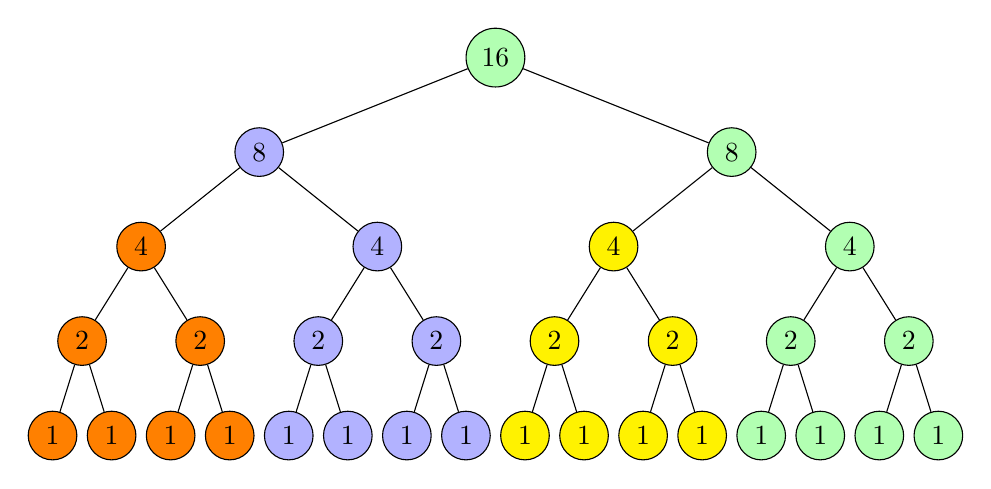
\begin{tikzpicture}[
                level distance=1.2cm,
                every node/.style={circle,draw,minimum size=6mm},
                level 1/.style={sibling distance=6cm},
                level 2/.style={sibling distance=3cm},
                level 3/.style={sibling distance=1.5cm},
                level 4/.style={sibling distance=0.75cm}
            ]

            \node[fill=green!30] {16}
            child {node[fill=blue!30] {8}
                    child {node[fill=orange] {4}
                            child {node[fill=orange] {2}
                                    child {node[fill=orange] {1}}
                                    child {node[fill=orange] {1}}
                                }
                            child {node[fill=orange] {2}
                                    child {node[fill=orange] {1}}
                                    child {node[fill=orange] {1}}
                                }
                        }
                    child {node[fill=blue!30] {4}
                            child {node[fill=blue!30] {2}
                                    child {node[fill=blue!30] {1}}
                                    child {node[fill=blue!30] {1}}
                                }
                            child {node[fill=blue!30] {2}
                                    child {node[fill=blue!30] {1}}
                                    child {node[fill=blue!30] {1}}
                                }
                        }
                }
            child {node[fill=green!30] {8}
                    child {node[fill=yellow] {4}
                            child {node[fill=yellow] {2}
                                    child {node[fill=yellow] {1}}
                                    child {node[fill=yellow] {1}}
                                }
                            child {node[fill=yellow] {2}
                                    child {node[fill=yellow] {1}}
                                    child {node[fill=yellow] {1}}
                                }
                        }
                    child {node[fill=green!30] {4}
                            child {node[fill=green!30] {2}
                                    child {node[fill=green!30] {1}}
                                    child {node[fill=green!30] {1}}
                                }
                            child {node[fill=green!30] {2}
                                    child {node[fill=green!30] {1}}
                                    child {node[fill=green!30] {1}}
                                }
                        }
                };

        \end{tikzpicture}

    \end{frame}

    \begin{frame}{Maximal unbalancierter Binärbaum für $n = 4$, $p=2$, $e=1$}
        Tiefenbasierte Thread-Erzeugung Quicksort \textbf{Worst-Case}:
        \newline
        \newline
        \centering
        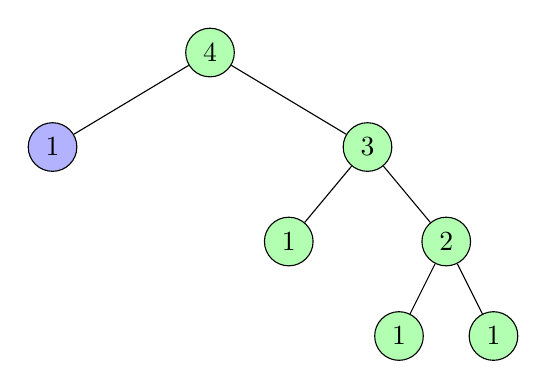
\begin{tikzpicture}[
                level distance=1.2cm,
                every node/.style={circle,draw,minimum size=6mm},
                level 1/.style={sibling distance=4cm},
                level 2/.style={sibling distance=2cm},
                level 3/.style={sibling distance=1.2cm}
            ]

            \node[fill=green!30] {4}
            child {node[fill=blue!30] {1}
                }
            child {node[fill=green!30] {3}
                    child {node[fill=green!30] {1}
                        }
                    child {node[fill=green!30] {2}
                            child {node[fill=green!30] {1}}
                            child {node[fill=green!30] {1}}
                        }
                };

        \end{tikzpicture}
    \end{frame}

    \begin{frame}{Maximal unbalancierter Binärbaum für $n = 4$, $p=2$}
        Worker-Thread-Variante Quicksort \textbf{Worst-Case}:
        \newline
        \newline
        \centering
        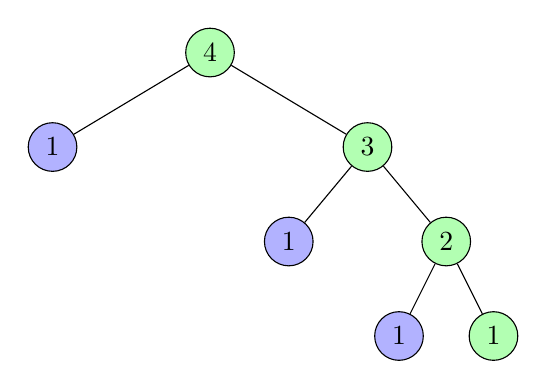
\begin{tikzpicture}[
                level distance=1.2cm,
                every node/.style={circle,draw,minimum size=6mm},
                level 1/.style={sibling distance=4cm},
                level 2/.style={sibling distance=2cm},
                level 3/.style={sibling distance=1.2cm}
            ]

            \node[fill=green!30] {4}
            child {node[fill=blue!30] {1}
                }
            child {node[fill=green!30] {3}
                    child {node[fill=blue!30] {1}
                        }
                    child {node[fill=green!30] {2}
                            child {node[fill=blue!30] {1}}
                            child {node[fill=green!30] {1}}
                        }
                };

        \end{tikzpicture}
    \end{frame}

    \begin{frame}{Maximal unbalancierter Binärbaum für $n = 4$, $p=2$}
        Worker-Thread-Variante Quicksort \textbf{Worst-Case}:
        \newline
        \newline
        \centering
        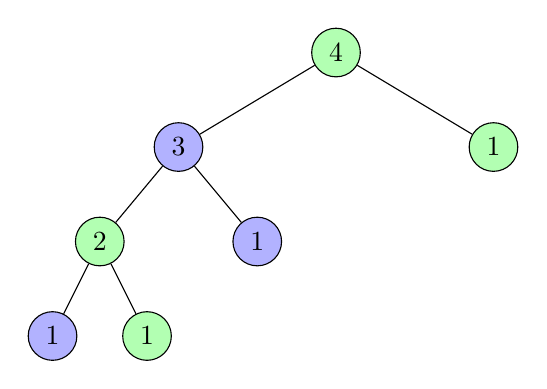
\begin{tikzpicture}[
                level distance=1.2cm,
                every node/.style={circle,draw,minimum size=6mm},
                level 1/.style={sibling distance=4cm},
                level 2/.style={sibling distance=2cm},
                level 3/.style={sibling distance=1.2cm}
            ]

            \node[fill=green!30] {4}
            child {node[fill=blue!30] {3}
                    child {node[fill=green!30] {2}
                            child {node[fill=blue!30] {1}}
                            child {node[fill=green!30] {1}}
                        }
                    child {node[fill=blue!30] {1}}
                }
            child {node[fill=green!30] {1}
                };

        \end{tikzpicture}
    \end{frame}

    \begin{frame}{Balancierter Binärbaum für $n = 16$, $p=4$}
        Worker-Thread-Variante Quicksort \textbf{Best-Case}:
        \newline
        \newline
        \centering
        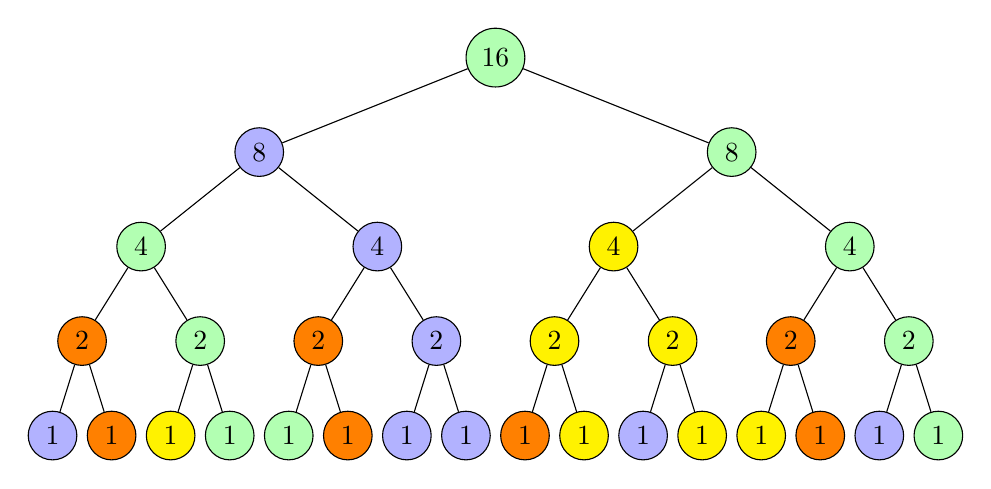
\begin{tikzpicture}[
                level distance=1.2cm,
                every node/.style={circle,draw,minimum size=6mm},
                level 1/.style={sibling distance=6cm},
                level 2/.style={sibling distance=3cm},
                level 3/.style={sibling distance=1.5cm},
                level 4/.style={sibling distance=0.75cm}
            ]

            \node[fill=green!30] {16}
            child {node[fill=blue!30] {8}
                    child {node[fill=green!30] {4}
                            child {node[fill=orange] {2}
                                    child {node[fill=blue!30] {1}}
                                    child {node[fill=orange] {1}}
                                }
                            child {node[fill=green!30] {2}
                                    child {node[fill=yellow] {1}}
                                    child {node[fill=green!30] {1}}
                                }
                        }
                    child {node[fill=blue!30] {4}
                            child {node[fill=orange] {2}
                                    child {node[fill=green!30] {1}}
                                    child {node[fill=orange] {1}}
                                }
                            child {node[fill=blue!30] {2}
                                    child {node[fill=blue!30] {1}}
                                    child {node[fill=blue!30]{1}}
                                }
                        }
                }
            child {node[fill=green!30] {8}
                    child {node[fill=yellow] {4}
                            child {node[fill=yellow] {2}
                                    child {node[fill=orange] {1}}
                                    child {node[fill=yellow] {1}}
                                }
                            child {node[fill=yellow] {2}
                                    child {node[fill=blue!30] {1}}
                                    child {node[fill=yellow] {1}}
                                }
                        }
                    child {node[fill=green!30] {4}
                            child {node[fill=orange] {2}
                                    child {node[fill=yellow] {1}}
                                    child {node[fill=orange] {1}}
                                }
                            child {node[fill=green!30] {2}
                                    child {node[fill=blue!30] {1}}
                                    child {node[fill=green!30] {1}}
                                }
                        }
                };

        \end{tikzpicture}

    \end{frame}

    \begin{frame}{Balancierter Binärbaum für $n = 16$, $p=4$}
        Worker-Thread-Variante Mergesort:
        \newline
        \newline
        \centering
        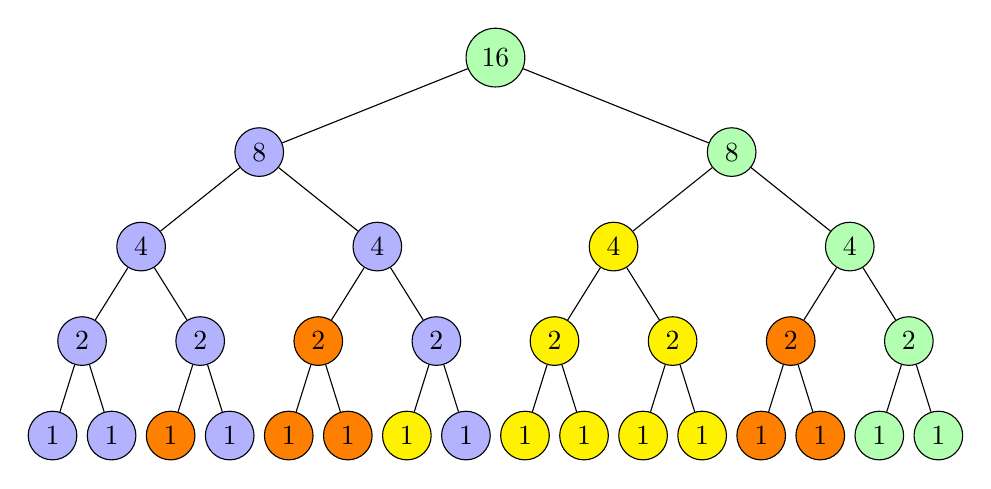
\begin{tikzpicture}[
                level distance=1.2cm,
                every node/.style={circle,draw,minimum size=6mm},
                level 1/.style={sibling distance=6cm},
                level 2/.style={sibling distance=3cm},
                level 3/.style={sibling distance=1.5cm},
                level 4/.style={sibling distance=0.75cm}
            ]

            \node[fill=green!30] {16}
            child {node[fill=blue!30] {8}
                    child {node[fill=blue!30] {4}
                            child {node[fill=blue!30] {2}
                                    child {node[fill=blue!30] {1}}
                                    child {node[fill=blue!30] {1}}
                                }
                            child {node[fill=blue!30] {2}
                                    child {node[fill=orange] {1}}
                                    child {node[fill=blue!30] {1}}
                                }
                        }
                    child {node[fill=blue!30] {4}
                            child {node[fill=orange] {2}
                                    child {node[fill=orange] {1}}
                                    child {node[fill=orange] {1}}
                                }
                            child {node[fill=blue!30] {2}
                                    child {node[fill=yellow] {1}}
                                    child {node[fill=blue!30] {1}}
                                }
                        }
                }
            child {node[fill=green!30] {8}
                    child {node[fill=yellow] {4}
                            child {node[fill=yellow] {2}
                                    child {node[fill=yellow] {1}}
                                    child {node[fill=yellow] {1}}
                                }
                            child {node[fill=yellow] {2}
                                    child {node[fill=yellow] {1}}
                                    child {node[fill=yellow] {1}}
                                }
                        }
                    child {node[fill=green!30] {4}
                            child {node[fill=orange] {2}
                                    child {node[fill=orange] {1}}
                                    child {node[fill=orange] {1}}
                                }
                            child {node[fill=green!30] {2}
                                    child {node[fill=green!30] {1}}
                                    child {node[fill=green!30] {1}}
                                }
                        }
                };

        \end{tikzpicture}

    \end{frame}

}

\newcommand{\BalancierterBinaerbaumNSechzehn}{
    \centering
    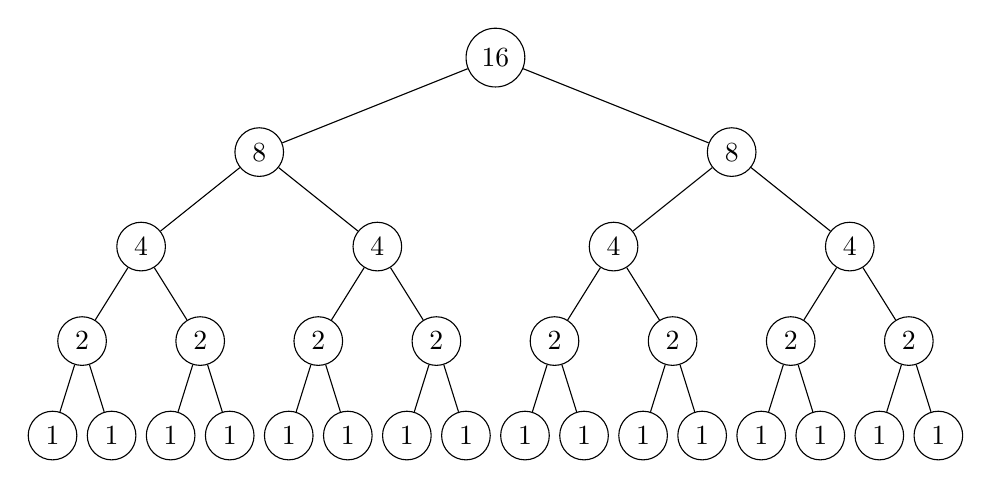
\begin{tikzpicture}[
            level distance=1.2cm,
            every node/.style={circle,draw,minimum size=6mm},
            level 1/.style={sibling distance=6cm},
            level 2/.style={sibling distance=3cm},
            level 3/.style={sibling distance=1.5cm},
            level 4/.style={sibling distance=0.75cm}
        ]

        \node {16}
        child {node {8}
                child {node {4}
                        child {node {2}
                                child {node {1}}
                                child {node {1}}
                            }
                        child {node {2}
                                child {node {1}}
                                child {node {1}}
                            }
                    }
                child {node {4}
                        child {node {2}
                                child {node {1}}
                                child {node {1}}
                            }
                        child {node {2}
                                child {node {1}}
                                child {node {1}}
                            }
                    }
            }
        child {node {8}
                child {node {4}
                        child {node {2}
                                child {node {1}}
                                child {node {1}}
                            }
                        child {node {2}
                                child {node {1}}
                                child {node {1}}
                            }
                    }
                child {node {4}
                        child {node {2}
                                child {node {1}}
                                child {node {1}}
                            }
                        child {node {2}
                                child {node {1}}
                                child {node {1}}
                            }
                    }
            };

    \end{tikzpicture}
}

\newcommand{\QuicksortWorstCaseBaum}{
    \centering
    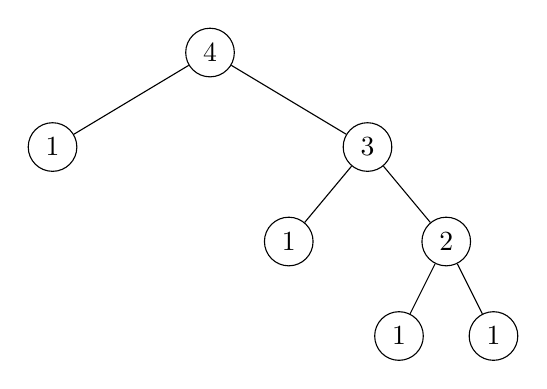
\begin{tikzpicture}[
            level distance=1.2cm,
            every node/.style={circle,draw,minimum size=6mm},
            level 1/.style={sibling distance=4cm},
            level 2/.style={sibling distance=2cm},
            level 3/.style={sibling distance=1.2cm}
        ]

        \node {4}
        child {node {1}
            }
        child {node {3}
                child {node {1}
                    }
                child {node {2}
                        child {node {1}}
                        child {node {1}}
                    }
            };

    \end{tikzpicture}
}

\newcommand{\HerleitungTnp}{
    \section{Herleitung T(n,p)}
    \begin{frame}{Herleitung T(n,p): Ausgangsdefinition}

        Gegeben ist die Rekursion:

        \[
            T(n,e)=
            \begin{cases}
                2\,T\!\left(\frac{n}{2},0\right)+n
                 & \text{falls } e=0 \\[8pt]
                T\!\left(\frac{n}{2},e-1\right)+n
                 & \text{falls } e>0
            \end{cases}
        \]

        Zusätzlich gilt:

        \[
            p = 2^e
        \]

    \end{frame}

    \begin{frame}{Herleitung T(n,p): Entfaltung der Rekursion (1. Schritt)}

        Für $e > 0$ gilt:

        \[
            T(n,e)=T\!\left(\frac{n}{2},e-1\right)+n
        \]

        Ein Einsetzen ergibt:

        \[
            T(n,e)
            =
            T\!\left(\frac{n}{4},e-2\right)
            +
            \frac{n}{2}
            +
            n
        \]

        Noch ein weiteres Einsetzen:

        \[
            T(n,e)
            =
            T\!\left(\frac{n}{8},e-3\right)
            +
            \frac{n}{4}
            +
            \frac{n}{2}
            +
            n
        \]

        Nach $e$ Schritten ergibt sich:

        \[
            T(n,e)
            =
            T\!\left(\frac{n}{2^e},0\right)
            +
            n
            \left(
            1+\frac12+\frac14+\dots+\frac1{2^{e-1}}
            \right)
        \]

    \end{frame}

    \begin{frame}{Herleitung T(n,p): Auswertung der geometrischen Reihe}

        Die Summe

        \[
            \left(
            1+\frac12+\frac14+\dots+\frac1{2^{e-1}}
            \right) = \sum_{i=0}^{e-1} \frac{1}{2^i}
        \]

        ist eine geometrische Reihe mit Quotient $\frac{1}{2}$.

        Sie ergibt:

        \[
            \sum_{i=0}^{e-1} \frac{1}{2^i}
            =
            2\left(1-\frac1{2^e}\right)
        \]

        Damit folgt:

        \[
            T(n,e)
            =
            T\!\left(\frac{n}{2^e},0\right)
            +
            2n\left(1-\frac1{2^e}\right)
        \]

    \end{frame}

    \begin{frame}{Herleitung T(n,p): Einsetzen des Basisfalls}

        Für $e=0$ gilt:

        \[
            T(n,0)=2T\!\left(\frac{n}{2},0\right)+n
        \]

        Dies entspricht der Rekursion von sequenziellem Mergesort.

        Bekannt ist:

        \[
            T(n,0)=n\log_2 n + n
        \]

        Ersetzen von $n$ durch $\frac{n}{2^e}$ ergibt:

        \[
            T\!\left(\frac{n}{2^e},0\right)
            =
            \frac{n}{2^e}
            \log_2\!\left(\frac{n}{2^e}\right)
            +
            \frac{n}{2^e}
        \]

        Einsetzen in $T(n,e)$ liefert:

        \[
            T(n,e)
            =
            \frac{n}{2^e}
            \log_2\!\left(\frac{n}{2^e}\right)
            +
            \frac{n}{2^e}
            +
            2n\left(1-\frac1{2^e}\right)
        \]

    \end{frame}

    \begin{frame}{Herleitung T(n,p): Substitution $p = 2^e$}

        Da gilt:

        \[
            p = 2^e
        \]

        folgt:

        \[
            \frac{n}{2^e} = \frac{n}{p}
        \]

        Damit ergibt sich:

        \[
            T(n,p)
            =
            \frac{n}{p}
            \log_2\!\left(\frac{n}{p}\right)
            +
            \frac{n}{p}
            +
            2n\left(1-\frac1{p}\right)
        \]

        Umsortiert erhält man:

        \[
            T(n,p)
            =
            2n\left(1-\frac1{p}\right)
            +
            \frac{n}{p}\log_2\!\left(\frac{n}{p}\right)
            +
            \frac{n}{p}
        \]

    \end{frame}
}

\newcommand{\alleFolien}{
    \HerleitungTnp
    \section*{Binärbaum}
    \begin{frame}{Balancierter Binärbaum für $n = 16$}
        \BalancierterBinaerbaumNSechzehn
    \end{frame}

    \begin{frame}{Balancierter Binärbaum für $n = 16$, $p=4$, $e=2$}

        \centering
        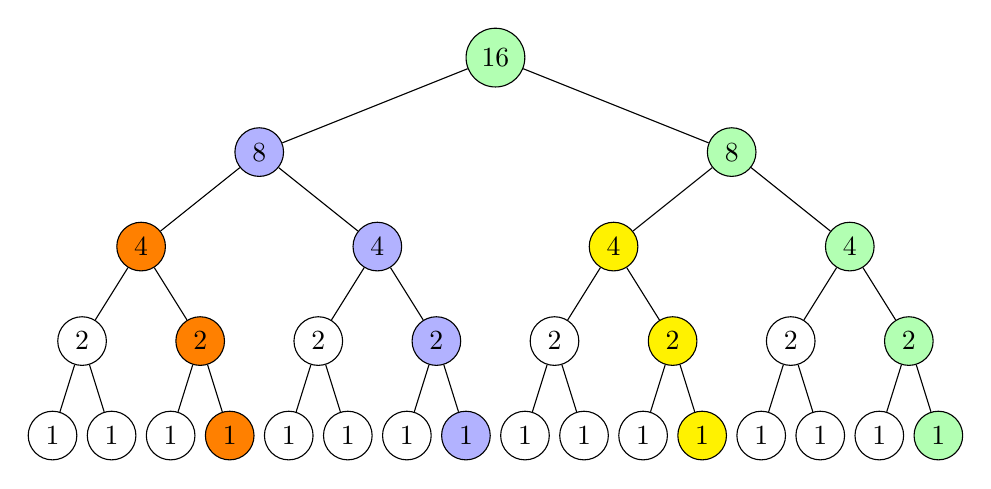
\begin{tikzpicture}[
                level distance=1.2cm,
                every node/.style={circle,draw,minimum size=6mm},
                level 1/.style={sibling distance=6cm},
                level 2/.style={sibling distance=3cm},
                level 3/.style={sibling distance=1.5cm},
                level 4/.style={sibling distance=0.75cm}
            ]

            \node[fill=green!30] {16}
            child {node[fill=blue!30] {8}
                    child {node[fill=orange] {4}
                            child {node {2}
                                    child {node {1}}
                                    child {node {1}}
                                }
                            child {node[fill=orange] {2}
                                    child {node {1}}
                                    child {node[fill=orange] {1}}
                                }
                        }
                    child {node[fill=blue!30] {4}
                            child {node {2}
                                    child {node {1}}
                                    child {node {1}}
                                }
                            child {node[fill=blue!30] {2}
                                    child {node {1}}
                                    child {node[fill=blue!30] {1}}
                                }
                        }
                }
            child {node[fill=green!30] {8}
                    child {node[fill=yellow] {4}
                            child {node {2}
                                    child {node {1}}
                                    child {node {1}}
                                }
                            child {node[fill=yellow] {2}
                                    child {node {1}}
                                    child {node[fill=yellow] {1}}
                                }
                        }
                    child {node[fill=green!30] {4}
                            child {node {2}
                                    child {node {1}}
                                    child {node {1}}
                                }
                            child {node[fill=green!30] {2}
                                    child {node {1}}
                                    child {node[fill=green!30] {1}}
                                }
                        }
                };

        \end{tikzpicture}

    \end{frame}

    \begin{frame}{Balancierter Binärbaum für $n = 16$, $p=4$, $e=2$}

        \centering
        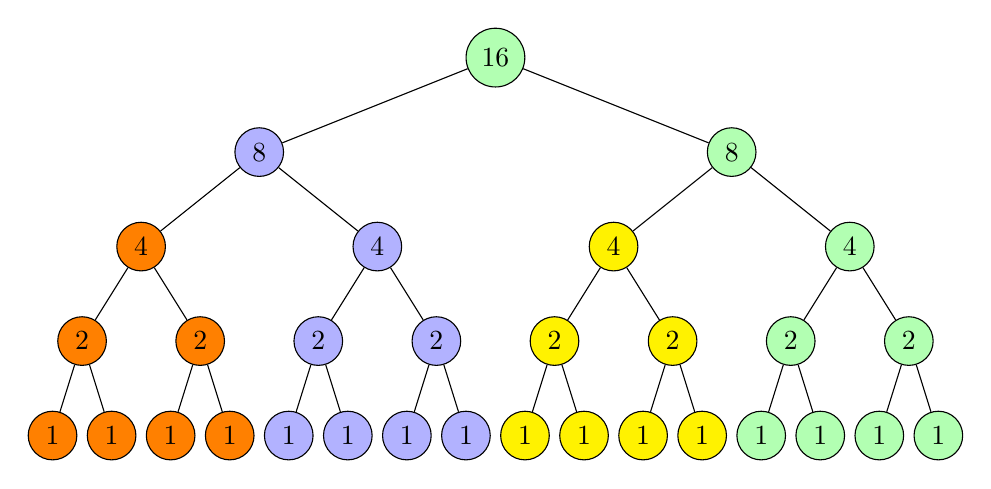
\begin{tikzpicture}[
                level distance=1.2cm,
                every node/.style={circle,draw,minimum size=6mm},
                level 1/.style={sibling distance=6cm},
                level 2/.style={sibling distance=3cm},
                level 3/.style={sibling distance=1.5cm},
                level 4/.style={sibling distance=0.75cm}
            ]

            \node[fill=green!30] {16}
            child {node[fill=blue!30] {8}
                    child {node[fill=orange] {4}
                            child {node[fill=orange] {2}
                                    child {node[fill=orange] {1}}
                                    child {node[fill=orange] {1}}
                                }
                            child {node[fill=orange] {2}
                                    child {node[fill=orange] {1}}
                                    child {node[fill=orange] {1}}
                                }
                        }
                    child {node[fill=blue!30] {4}
                            child {node[fill=blue!30] {2}
                                    child {node[fill=blue!30] {1}}
                                    child {node[fill=blue!30] {1}}
                                }
                            child {node[fill=blue!30] {2}
                                    child {node[fill=blue!30] {1}}
                                    child {node[fill=blue!30] {1}}
                                }
                        }
                }
            child {node[fill=green!30] {8}
                    child {node[fill=yellow] {4}
                            child {node[fill=yellow] {2}
                                    child {node[fill=yellow] {1}}
                                    child {node[fill=yellow] {1}}
                                }
                            child {node[fill=yellow] {2}
                                    child {node[fill=yellow] {1}}
                                    child {node[fill=yellow] {1}}
                                }
                        }
                    child {node[fill=green!30] {4}
                            child {node[fill=green!30] {2}
                                    child {node[fill=green!30] {1}}
                                    child {node[fill=green!30] {1}}
                                }
                            child {node[fill=green!30] {2}
                                    child {node[fill=green!30] {1}}
                                    child {node[fill=green!30] {1}}
                                }
                        }
                };

        \end{tikzpicture}

    \end{frame}

    \begin{frame}{Balancierter Binärbaum für $n = 16$, $p=4$}
        Worker-Thread-Variante Mergesort:
        \centering
        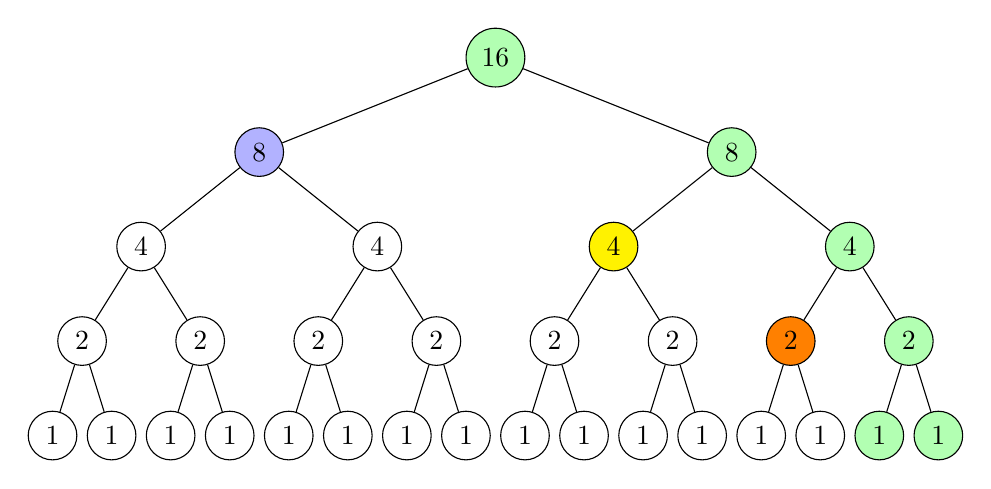
\begin{tikzpicture}[
                level distance=1.2cm,
                every node/.style={circle,draw,minimum size=6mm},
                level 1/.style={sibling distance=6cm},
                level 2/.style={sibling distance=3cm},
                level 3/.style={sibling distance=1.5cm},
                level 4/.style={sibling distance=0.75cm}
            ]

            \node[fill=green!30] {16}
            child {node[fill=blue!30] {8}
                    child {node {4}
                            child {node {2}
                                    child {node {1}}
                                    child {node {1}}
                                }
                            child {node {2}
                                    child {node {1}}
                                    child {node {1}}
                                }
                        }
                    child {node {4}
                            child {node {2}
                                    child {node {1}}
                                    child {node {1}}
                                }
                            child {node {2}
                                    child {node {1}}
                                    child {node {1}}
                                }
                        }
                }
            child {node[fill=green!30] {8}
                    child {node[fill=yellow] {4}
                            child {node {2}
                                    child {node {1}}
                                    child {node {1}}
                                }
                            child {node {2}
                                    child {node {1}}
                                    child {node {1}}
                                }
                        }
                    child {node[fill=green!30] {4}
                            child {node[fill=orange] {2}
                                    child {node {1}}
                                    child {node {1}}
                                }
                            child {node[fill=green!30] {2}
                                    child {node[fill=green!30] {1}}
                                    child {node[fill=green!30] {1}}
                                }
                        }
                };

        \end{tikzpicture}

    \end{frame}

    \begin{frame}{Balancierter Binärbaum für $n = 16$, $p=4$}
        Worker-Thread-Variante Mergesort:
        \centering
        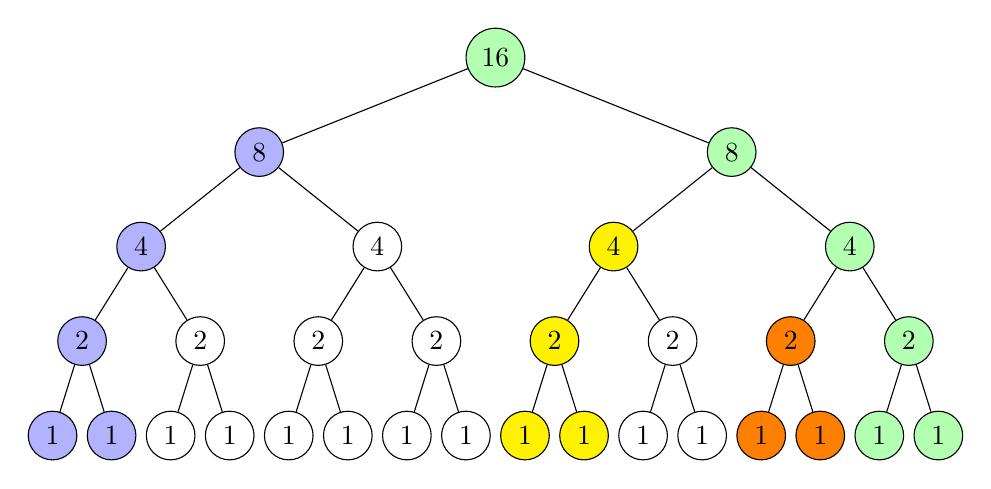
\begin{tikzpicture}[
                level distance=1.2cm,
                every node/.style={circle,draw,minimum size=6mm},
                level 1/.style={sibling distance=6cm},
                level 2/.style={sibling distance=3cm},
                level 3/.style={sibling distance=1.5cm},
                level 4/.style={sibling distance=0.75cm}
            ]

            \node[fill=green!30] {16}
            child {node[fill=blue!30] {8}
                    child {node[fill=blue!30] {4}
                            child {node[fill=blue!30] {2}
                                    child {node[fill=blue!30] {1}}
                                    child {node[fill=blue!30] {1}}
                                }
                            child {node {2}
                                    child {node {1}}
                                    child {node {1}}
                                }
                        }
                    child {node {4}
                            child {node {2}
                                    child {node {1}}
                                    child {node {1}}
                                }
                            child {node {2}
                                    child {node {1}}
                                    child {node {1}}
                                }
                        }
                }
            child {node[fill=green!30] {8}
                    child {node[fill=yellow] {4}
                            child {node[fill=yellow] {2}
                                    child {node[fill=yellow] {1}}
                                    child {node[fill=yellow] {1}}
                                }
                            child {node {2}
                                    child {node {1}}
                                    child {node {1}}
                                }
                        }
                    child {node[fill=green!30] {4}
                            child {node[fill=orange] {2}
                                    child {node[fill=orange] {1}}
                                    child {node[fill=orange] {1}}
                                }
                            child {node[fill=green!30] {2}
                                    child {node[fill=green!30] {1}}
                                    child {node[fill=green!30] {1}}
                                }
                        }
                };

        \end{tikzpicture}

    \end{frame}

    \begin{frame}{Balancierter Binärbaum für $n = 16$, $p=4$}
        Worker-Thread-Variante Mergesort:
        \centering
        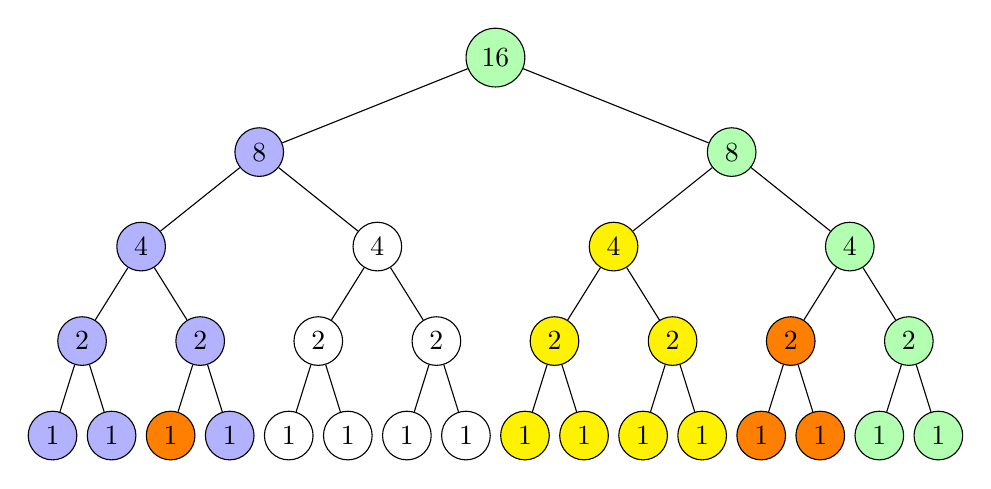
\begin{tikzpicture}[
                level distance=1.2cm,
                every node/.style={circle,draw,minimum size=6mm},
                level 1/.style={sibling distance=6cm},
                level 2/.style={sibling distance=3cm},
                level 3/.style={sibling distance=1.5cm},
                level 4/.style={sibling distance=0.75cm}
            ]

            \node[fill=green!30] {16}
            child {node[fill=blue!30] {8}
                    child {node[fill=blue!30] {4}
                            child {node[fill=blue!30] {2}
                                    child {node[fill=blue!30] {1}}
                                    child {node[fill=blue!30] {1}}
                                }
                            child {node[fill=blue!30] {2}
                                    child {node[fill=orange] {1}}
                                    child {node[fill=blue!30] {1}}
                                }
                        }
                    child {node {4}
                            child {node {2}
                                    child {node {1}}
                                    child {node {1}}
                                }
                            child {node {2}
                                    child {node {1}}
                                    child {node {1}}
                                }
                        }
                }
            child {node[fill=green!30] {8}
                    child {node[fill=yellow] {4}
                            child {node[fill=yellow] {2}
                                    child {node[fill=yellow] {1}}
                                    child {node[fill=yellow] {1}}
                                }
                            child {node[fill=yellow] {2}
                                    child {node[fill=yellow] {1}}
                                    child {node[fill=yellow] {1}}
                                }
                        }
                    child {node[fill=green!30] {4}
                            child {node[fill=orange] {2}
                                    child {node[fill=orange] {1}}
                                    child {node[fill=orange] {1}}
                                }
                            child {node[fill=green!30] {2}
                                    child {node[fill=green!30] {1}}
                                    child {node[fill=green!30] {1}}
                                }
                        }
                };

        \end{tikzpicture}

    \end{frame}

    \begin{frame}{Balancierter Binärbaum für $n = 16$, $p=4$}
        Worker-Thread-Variante Mergesort:
        \centering
        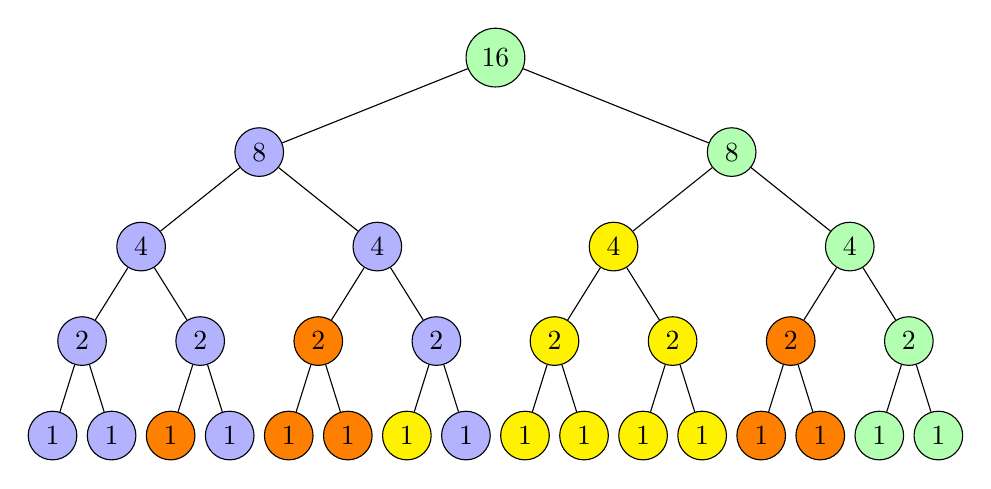
\begin{tikzpicture}[
                level distance=1.2cm,
                every node/.style={circle,draw,minimum size=6mm},
                level 1/.style={sibling distance=6cm},
                level 2/.style={sibling distance=3cm},
                level 3/.style={sibling distance=1.5cm},
                level 4/.style={sibling distance=0.75cm}
            ]

            \node[fill=green!30] {16}
            child {node[fill=blue!30] {8}
                    child {node[fill=blue!30] {4}
                            child {node[fill=blue!30] {2}
                                    child {node[fill=blue!30] {1}}
                                    child {node[fill=blue!30] {1}}
                                }
                            child {node[fill=blue!30] {2}
                                    child {node[fill=orange] {1}}
                                    child {node[fill=blue!30] {1}}
                                }
                        }
                    child {node[fill=blue!30] {4}
                            child {node[fill=orange] {2}
                                    child {node[fill=orange] {1}}
                                    child {node[fill=orange] {1}}
                                }
                            child {node[fill=blue!30] {2}
                                    child {node[fill=yellow] {1}}
                                    child {node[fill=blue!30] {1}}
                                }
                        }
                }
            child {node[fill=green!30] {8}
                    child {node[fill=yellow] {4}
                            child {node[fill=yellow] {2}
                                    child {node[fill=yellow] {1}}
                                    child {node[fill=yellow] {1}}
                                }
                            child {node[fill=yellow] {2}
                                    child {node[fill=yellow] {1}}
                                    child {node[fill=yellow] {1}}
                                }
                        }
                    child {node[fill=green!30] {4}
                            child {node[fill=orange] {2}
                                    child {node[fill=orange] {1}}
                                    child {node[fill=orange] {1}}
                                }
                            child {node[fill=green!30] {2}
                                    child {node[fill=green!30] {1}}
                                    child {node[fill=green!30] {1}}
                                }
                        }
                };

        \end{tikzpicture}

    \end{frame}


    \begin{frame}{Balancierter Binärbaum für $n = 16$, $p=4$}
        Worker-Thread-Variante Quicksort \textbf{Best-Case}:
        \centering
        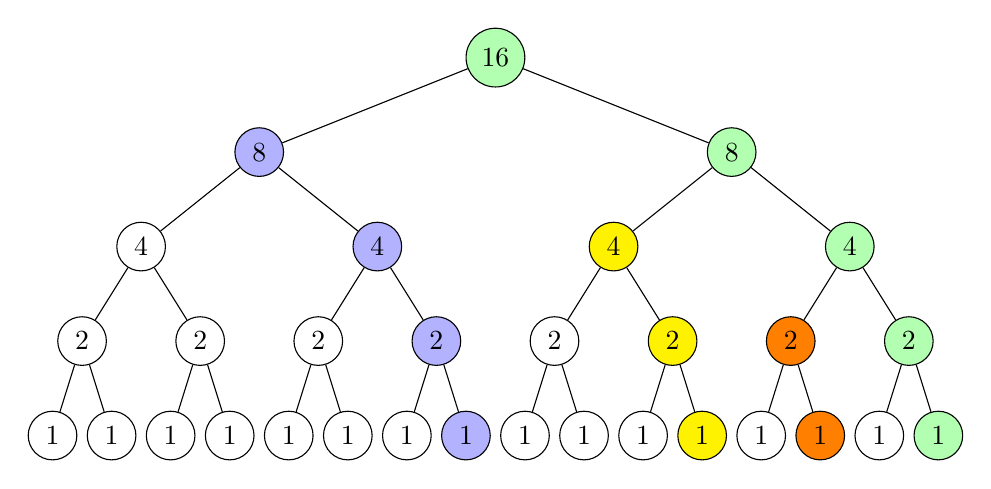
\begin{tikzpicture}[
                level distance=1.2cm,
                every node/.style={circle,draw,minimum size=6mm},
                level 1/.style={sibling distance=6cm},
                level 2/.style={sibling distance=3cm},
                level 3/.style={sibling distance=1.5cm},
                level 4/.style={sibling distance=0.75cm}
            ]

            \node[fill=green!30] {16}
            child {node[fill=blue!30] {8}
                    child {node {4}
                            child {node {2}
                                    child {node {1}}
                                    child {node {1}}
                                }
                            child {node {2}
                                    child {node {1}}
                                    child {node {1}}
                                }
                        }
                    child {node[fill=blue!30] {4}
                            child {node {2}
                                    child {node {1}}
                                    child {node {1}}
                                }
                            child {node[fill=blue!30] {2}
                                    child {node {1}}
                                    child {node [fill=blue!30]{1}}
                                }
                        }
                }
            child {node[fill=green!30] {8}
                    child {node[fill=yellow] {4}
                            child {node {2}
                                    child {node {1}}
                                    child {node {1}}
                                }
                            child {node[fill=yellow] {2}
                                    child {node {1}}
                                    child {node[fill=yellow] {1}}
                                }
                        }
                    child {node[fill=green!30] {4}
                            child {node[fill=orange] {2}
                                    child {node {1}}
                                    child {node[fill=orange] {1}}
                                }
                            child {node[fill=green!30] {2}
                                    child {node {1}}
                                    child {node[fill=green!30] {1}}
                                }
                        }
                };

        \end{tikzpicture}

    \end{frame}

    \begin{frame}{Balancierter Binärbaum für $n = 16$, $p=4$}
        Worker-Thread-Variante Quicksort \textbf{Best-Case}:
        \centering
        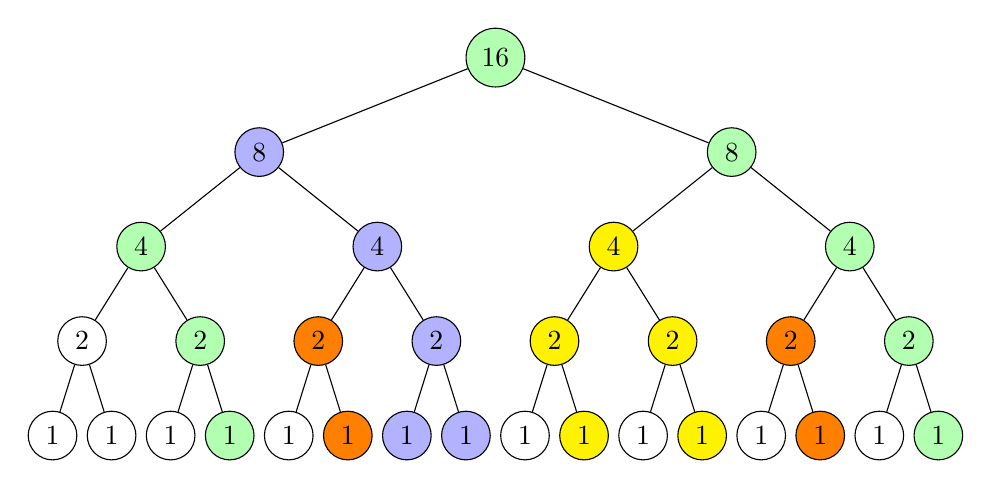
\begin{tikzpicture}[
                level distance=1.2cm,
                every node/.style={circle,draw,minimum size=6mm},
                level 1/.style={sibling distance=6cm},
                level 2/.style={sibling distance=3cm},
                level 3/.style={sibling distance=1.5cm},
                level 4/.style={sibling distance=0.75cm}
            ]

            \node[fill=green!30] {16}
            child {node[fill=blue!30] {8}
                    child {node[fill=green!30] {4}
                            child {node {2}
                                    child {node {1}}
                                    child {node {1}}
                                }
                            child {node[fill=green!30] {2}
                                    child {node {1}}
                                    child {node[fill=green!30] {1}}
                                }
                        }
                    child {node[fill=blue!30] {4}
                            child {node[fill=orange] {2}
                                    child {node {1}}
                                    child {node[fill=orange] {1}}
                                }
                            child {node[fill=blue!30] {2}
                                    child {node[fill=blue!30] {1}}
                                    child {node[fill=blue!30]{1}}
                                }
                        }
                }
            child {node[fill=green!30] {8}
                    child {node[fill=yellow] {4}
                            child {node[fill=yellow] {2}
                                    child {node {1}}
                                    child {node[fill=yellow] {1}}
                                }
                            child {node[fill=yellow] {2}
                                    child {node {1}}
                                    child {node[fill=yellow] {1}}
                                }
                        }
                    child {node[fill=green!30] {4}
                            child {node[fill=orange] {2}
                                    child {node {1}}
                                    child {node[fill=orange] {1}}
                                }
                            child {node[fill=green!30] {2}
                                    child {node {1}}
                                    child {node[fill=green!30] {1}}
                                }
                        }
                };

        \end{tikzpicture}

    \end{frame}

    \begin{frame}{Maximal unbalancierter Binärbaum für $n = 4$, $p=2$}
        Worker-Thread-Variante Quicksort \textbf{Worst-Case}:
        \centering
        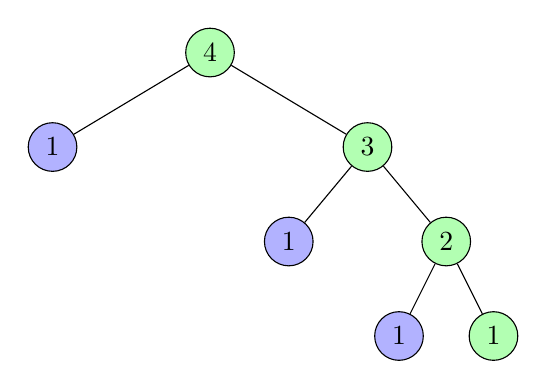
\begin{tikzpicture}[
                level distance=1.2cm,
                every node/.style={circle,draw,minimum size=6mm},
                level 1/.style={sibling distance=4cm},
                level 2/.style={sibling distance=2cm},
                level 3/.style={sibling distance=1.2cm}
            ]

            \node[fill=green!30] {4}
            child {node[fill=blue!30] {1}
                }
            child {node[fill=green!30] {3}
                    child {node[fill=blue!30] {1}
                        }
                    child {node[fill=green!30] {2}
                            child {node[fill=blue!30] {1}}
                            child {node[fill=green!30] {1}}
                        }
                };

        \end{tikzpicture}
    \end{frame}

    \begin{frame}{Maximal unbalancierter Binärbaum für $n = 4$, $p=2$}
        Worker-Thread-Variante Quicksort \textbf{Worst-Case}:
        \centering
        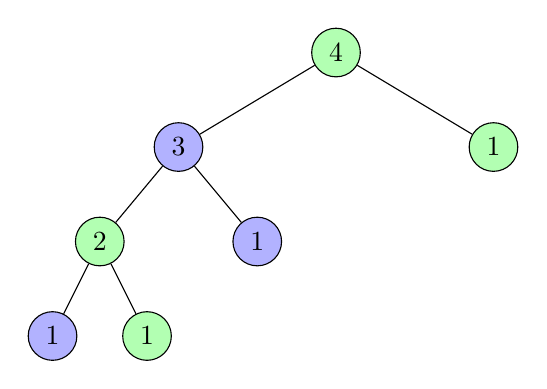
\begin{tikzpicture}[
                level distance=1.2cm,
                every node/.style={circle,draw,minimum size=6mm},
                level 1/.style={sibling distance=4cm},
                level 2/.style={sibling distance=2cm},
                level 3/.style={sibling distance=1.2cm}
            ]

            \node[fill=green!30] {4}
            child {node[fill=blue!30] {3}
                    child {node[fill=green!30] {2}
                            child {node[fill=blue!30] {1}}
                            child {node[fill=green!30] {1}}
                        }
                    child {node[fill=blue!30] {1}}
                }
            child {node[fill=green!30] {1}
                };

        \end{tikzpicture}
    \end{frame}
}